\documentclass{article}
\usepackage{amsmath}
\usepackage{esint}
\usepackage[utf8]{inputenc}
\usepackage{listings}
\usepackage{graphicx}
\usepackage{float}
\graphicspath{{/home/david/Documents/}}
\lstset{frame=single}
\linespread{1.5}
\usepackage[dvipsnames]{xcolor}



\begin{document}
	\title{INF 1400 - Oppsummering}
	\author{Dawid Kuleczko}
	\maketitle	
	
	\section*{Temaer:}
	\subsection*{Digital representasjon og binær logikk}
	\subsection*{Boolsk algebra}
	\subsection*{Karnaugh diagram}
	\subsection*{Kobinatorisk logikk}
	\subsection*{Sekvensiell logikk}
	\subsection*{Tilstandsmaskiner}
	\subsection*{Datamaskinarkitektur}
	\subsection*{CMOS}
	\quad
	
	\section*{Digital representasjon og binær logikk:}
	\subsection*{Tallsystemer:}
	
	I dette kurset skal vi legge spesielt vekt på binære tall, men heksadesimale tall og octale tall, samt tall fra andre tallsystemer, kan også forekomme.
	
	Til daglig bruker vi desimal, altså 10-tallsystemet. Et desimalt tall er representert ved symbolene fra 0 til 9.
	
	eks. $(951)_{dec} = 9 \cdot 10^2 + 5 \cdot 10^1 + 1 \cdot 10^0$
	
	Et binært tall er representert ved symbolene 
	0 og 1.
	
	eks. $ (101)_{bin} = 1 \cdot 2^2 + 0 \cdot 2^1 + 1 \cdot 2^0$
	
	Et heksadesimalt tall er representert ved symbolene 
	fra 0 til F der tallene etter 9 er:
	10 = A
	11 = B
	12 = C
	13 = D
	14 = E
	15 = F
	
	eks. $(5BF)_{hex} = 5 \cdot 16^2 + 11 \cdot 16^1 + 15 \cdot 16^0$ 
	
	Et oktalt tall er representert ved symbolene fra 0 til 8.
	
	eks. $(853)_{oct} = 8 \cdot 8^2 + 5 \cdot 8^1 + 3 \cdot 3^0$

	\subsection*{Konvertering:}
	
	\subsubsection*{Konvertering fra grunntall r til desimaltall:}
	Generelt:
	$(...a_2 a_1 a_0 , a_{-1} a_{-2}...) = ... + a_2 \cdot r^2 + a_1 \cdot r^1 + a_0 \cdot r^0 , a_{-1} \cdot r^{-1} a_{-2} \cdot r^{-2} + ..$
	
	eks.
	$(1A5,1C)_{16} = 1 \cdot 16^2 + A \cdot 16^1 + 5 \cdot 16^0 + 1 \cdot 16^{-1} + 12 \cdot 16^{-2} = (421,109375)_{10}$
	
	
	
	\subsubsection*{Konvertering av desimal til binær:}
	
	Eks. $(23)_{10}$
	$$ 23/2 = 11 + 1/2 \qquad a_0 = 1 $$
	$$ 11/2 = 5 + 1/2 \qquad a_1 = 1 $$
	$$ 5/2 = 2 + 1/2 \qquad a_2 = 1 $$	
	$$ 2/2 = 1 + 0/2 \qquad a_3 = 0 
	$$
	$$1/2 = 0 + 1/2 \qquad a_4 = 1
	$$
	
	Vi leser det binære tallet nedfra $(10111)_{2}$
	
	
	\subsubsection*{Konvertering fra desimal til grunntall “r”:}
	Samme måte som over bare med "r" isteden for 2.
	
	Eks. $(12)_{10}$ til 3-tallsystemet:
	
	$$ 12/3 = 4 + 0/3 \qquad a_0 = 0$$
	$$ 4/3 = 1 + 1/3 \qquad a_1 = 1$$
	$$ 1/3 = 0 + 1/3 \qquad a_2 = 1 $$
	
	Tallet blir da $(110)_3$ i 3 tallsystemet.
	
	\subsubsection*{Sannhetstabell:}
		
	\begin{figure}[H]
		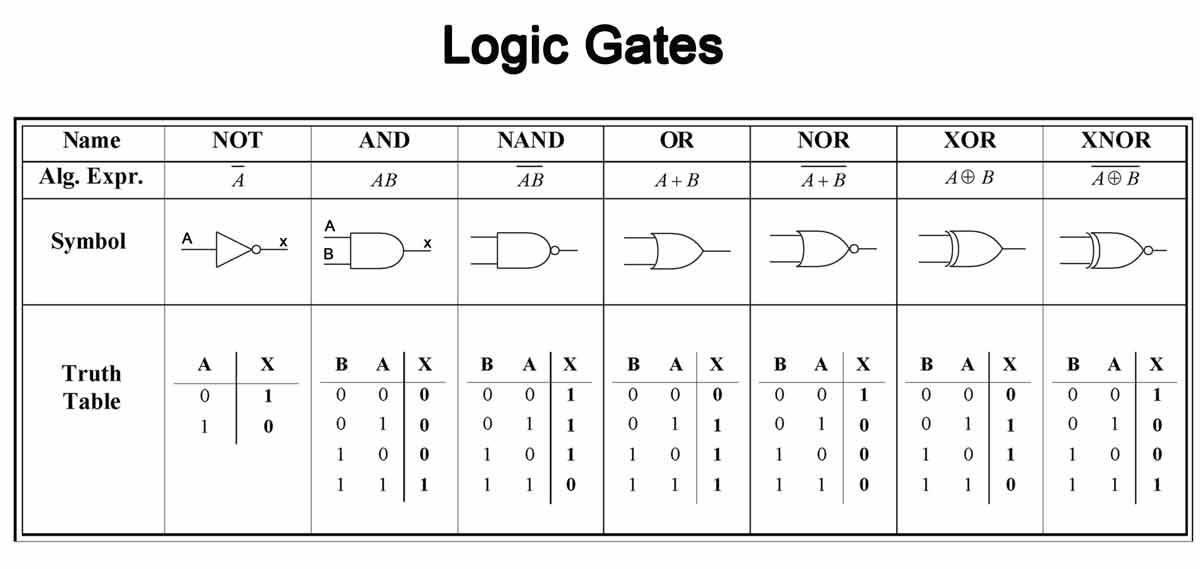
\includegraphics[scale=0.35]{GATES.jpg}
		\caption{Logiske porter}
	\end{figure}
	
	\begin{figure}[H]
		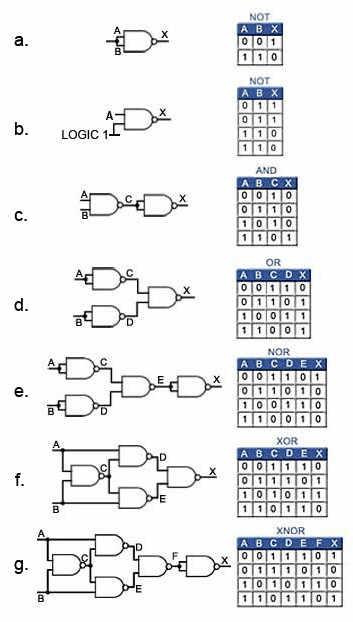
\includegraphics{NAND.jpg}
		\caption{Logiske porter som 2 inputs NAND-porter}
	\end{figure}
	
	\subsection*{Huntington's postulater}
	\begin{figure}[H]
		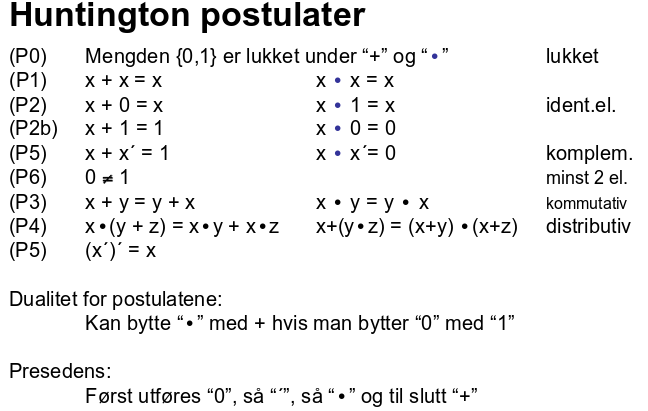
\includegraphics[scale=0.35]{Huntington.png}
		\caption{Huntington's postulater}
	\end{figure}
	
	
	\section*{Boolsk algebra:}
	
	\begin{figure}[H]
		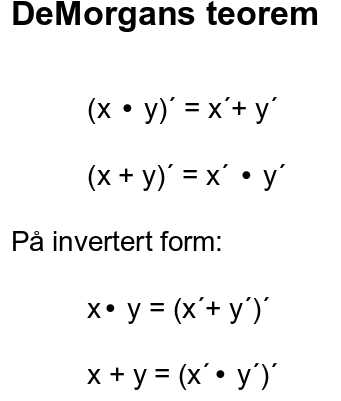
\includegraphics[scale=0.4]{DeMorgan.png}
		\caption{DeMorgans teorem}
	\end{figure}
	
	\begin{figure}[H]
		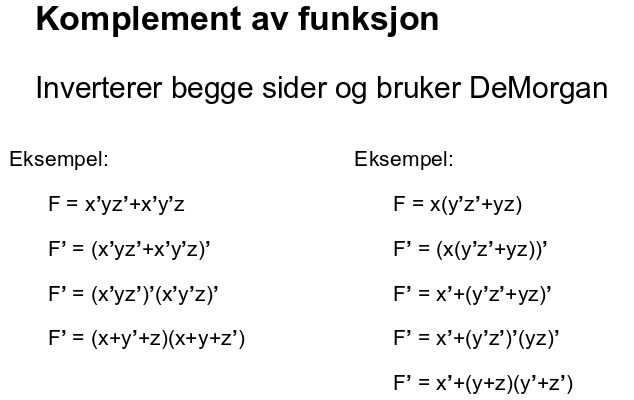
\includegraphics[scale=0.55]{Komplement.png}
		\caption{Komplement av funkson}
	\end{figure}
	
	\begin{figure}[H]
		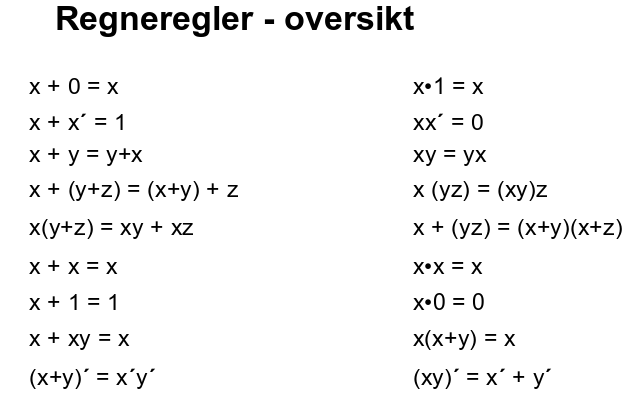
\includegraphics[scale=0.6]{Regneregler.png}
		\caption{Regne regler for boolsk algebra}
	\end{figure}
	
	\subsection*{Boolske funksjoner med sannhetstabell}
	En boolsk funksjon kan visualiseres i en 
	sannhetstabell.
	En gitt	funksjon har kun en	sannhetstabell 
	Men, en gitt sannhetstabell har uendelig mange funksjonsuttrykk.
	
	\textbf{Eksempel: F = x + y' z}
	
		\begin{center}
			\begin{tabular}{|c|c|}
				\hline
				XYZ & F \\ \hline
				000 & 0  \\ \hline
				001 & 1  \\ \hline 
				010 & 0  \\ \hline
				011 & 0  \\ \hline 
				100 & 1  \\ \hline
				101 & 1  \\ \hline
				110 & 1  \\ \hline
				111 & 1  \\ \hline
				
			\end{tabular}
		\end{center}
	
	
	\subsection*{Forenkling av uttryk}
	En funksjon kan forenkles ved regneregler for å gjøre den lettere å håndere og implementere.
	
	\begin{figure}[H]
		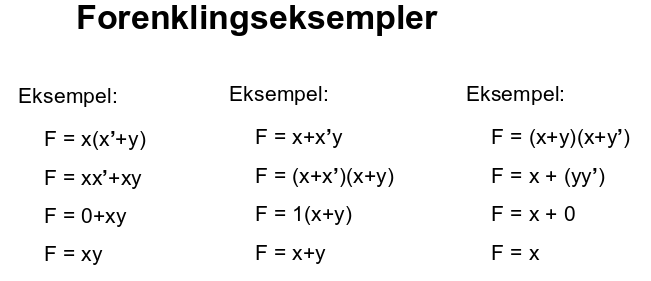
\includegraphics[scale=0.6]{Forenkling.png}
		\caption{Forenklingseksempler av noen funksjoner}
	\end{figure}
	
	\begin{figure}[H]
		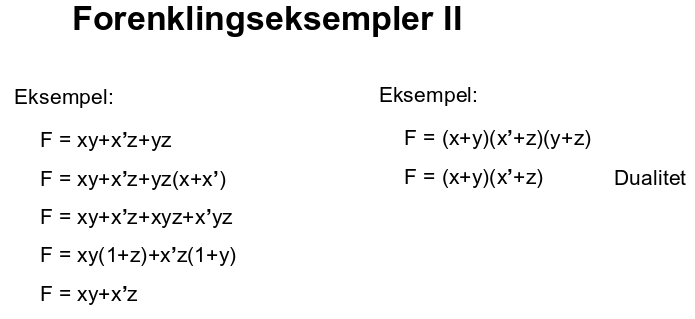
\includegraphics[scale=0.6]{Forenkling2.png}
		\caption{Forenklingseksempler av noen funksjoner}
	\end{figure}
	
	\subsection*{Maksterm/Minterm}
	
	\begin{figure}[H]
		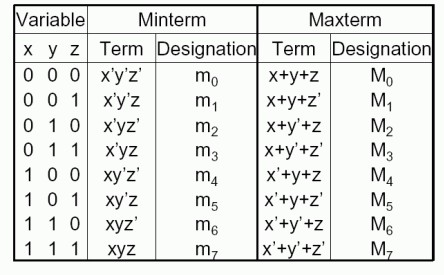
\includegraphics[scale=0.8]{maksmin.jpg}
		\caption{Tabell for minterm og maksterm}
	\end{figure}
	
	Mintermer har notasjon $m_x$
	
	$F\textcolor{Violet}{(x,y,z)} = \sum\textcolor{Violet}{(m_3, m_6)} = \sum\textcolor{Violet}{(3, 6)} = \textcolor{Violet}{ x'yz' + xyz'} $
	
	Makstermer har notasjon $M_x$
	
	$F\textcolor{Violet}{(x,y,z)} = \Pi \textcolor{Violet}{(M_3, M_6)} = \Pi \textcolor{Violet}{(3, 6)} = \textcolor{Violet}{(x+y'+z')(x'+y'+z)} $
	
	\subsubsection*{Minterm:}
	I en funksjon kan en binær variabel x opptre som x eller x'.	En funksjon kan være gitt på “sum av produkt” form.
	Eksempel: F = xy + xy' + x
	
	Hvert “produktledd” som inneholder alle variablene kalles en minterm. For to variable finnes det 4 forskjellige mintermer: xy + xy' + x'y + x'y'
	For 3 variable finnes det $2^3$ forskjellige mintermer. 
	
	Hvis man generer en funksjon ut i fra sannhetstabellen får man en sum av mintermer
	
	Eksempel:  F = \textcolor{Aquamarine}{x'y'z} + \textcolor{BurntOrange}{xy'z'} + \textcolor{WildStrawberry}{xyz'}
	
	
	\begin{center}
		\begin{tabular}{|c|c|}
			\hline
			XYZ & F \\ \hline
			000 & 0  \\ \hline
			001 & \color{Aquamarine}1  \\ \hline 
			010 & 0  \\ \hline
			011 & 0  \\ \hline 
			100 & \color{BurntOrange}1  \\ \hline
			101 & 0  \\ \hline
			110 & \color{WildStrawberry}1  \\ \hline
			111 & 0  \\ \hline
			
		\end{tabular}
	\end{center}
	
	En sannhetstabell kan sees på som en liste av mintermer.
	
	\subsubsection*{Maksterm:}
	
	En funksjon kan være gitt på “produkt av sum” form.
	
	Eksempel: F = (x+y)(x+y')y 
	Hvert "summeledd" som inneholder alle variablene kalles maksterm.
	
	For to variable finnes det 4 forskjellige makstermer:
	(x'y)(x+y')(x'+y)(x'+y')
	
	For n variable finnes det $2^n$ forskjellige makstermer.
	
	\subsection*{Designprosedyre }
	
	Det er ikke alltid at det enkleste funksjonsuttrykket resulterer i den enkleste port-implementasjonen.
	
	Ved forenkling på portnivå må man vite hvilke porter man har til rådighet, og så justere funksjonsuttrykket mot dette. (håndverk) 
	
	\textbf{Generell design	prosedyre}
	
	1.Bestem hvilke signal som er innganger og 
	utganger
	
	2.Sett opp sannhetstabell for alle 
	inngangskombinasjoner
	
	3.Generer funksjonsuttrykket som sum av 
	mintermer 
	
	4.Tilpass / forenkle funksjonsuttrykket mot 
	aktuelle porter 
	
	\section*{Karnaugh diagram:}
	Grafisk metode for forenkling av Boolske uttryk
	\begin{figure}[H]
		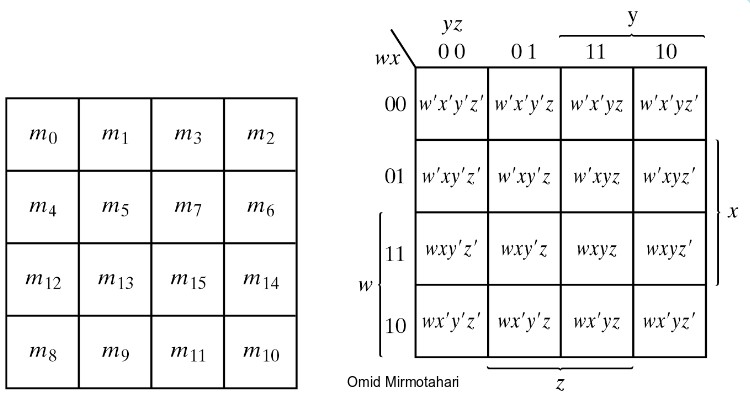
\includegraphics[scale = 0.6]{KarnaD.jpg}
		\caption{Karnaugh diagram med mintermene}
	\end{figure}
	
	\begin{figure}[H]
		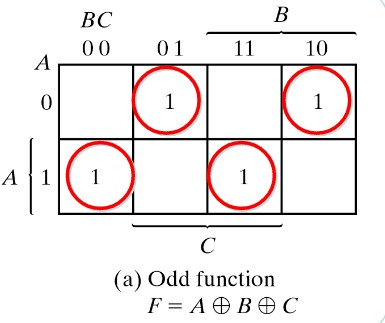
\includegraphics[scale = 0.6]{XOR.jpg}
		\caption{XOR}
	\end{figure}
	
	\begin{figure}[H]
		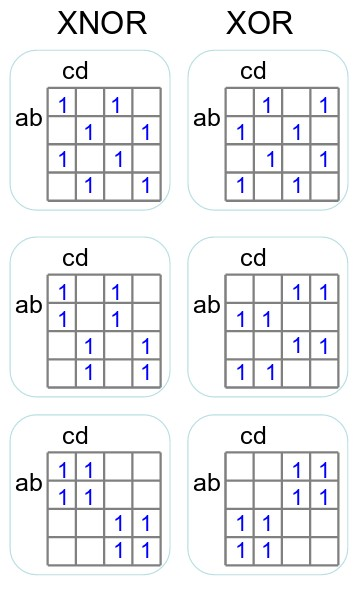
\includegraphics[scale = 0.7]{X.jpg}
		\caption{XNOR og XOR}
	\end{figure}
	
	
	\section*{Kobinatorisk logikk:}
	
	\subsection*{Binær addisjon:}
	 Prosedyren for binær addisjon er identisk med prosedyren for desimal addisjon:
	 
	 Eks: 
	 $\begin{bmatrix}
	 0 1 0 1 \\
	 1 0 1 1 & + \\
	 ------- \\
	 1 0 0 0 0
	 \end{bmatrix}$
	5 + 11 = 16
	\subsection*{Binær substraksjon:}
	\begin{figure}[H]
		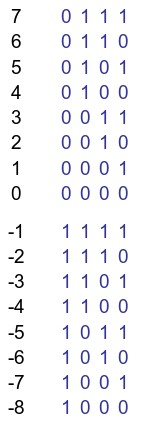
\includegraphics[scale = 0.7]{Nega.jpg}
		\caption{Representasjon av binære negative tall}
	\end{figure}
	
	For å substrahere negative binære tall, bruker man toerkomplement metoden.
	
	Det tallet som skal substraherers med må inverteres og plusses på 1, deretter skal det plusses med den andre tallet. Tallet til overs går ut.
	
	Eks: 
	$\begin{bmatrix}
	1 1 0 1 \\
	1 0 1 1 & -\\
	------- \\
	\end{bmatrix}$ 
	$\begin{bmatrix}
	1 1 0 1 \\
	0 1 0 1 & +\\
	------- \\
	(1) 0 0 1 0
	\end{bmatrix}$
	13-11 = 2
	
	13+5=18 = 1 0 0 1 0
	
	\subsection*{Binære addere:}
	\subsubsection*{Halvadder:}
	Halvaddere tar ikke mente inn.
	
	Halvadder implementasjon
	\begin{figure}[H]
		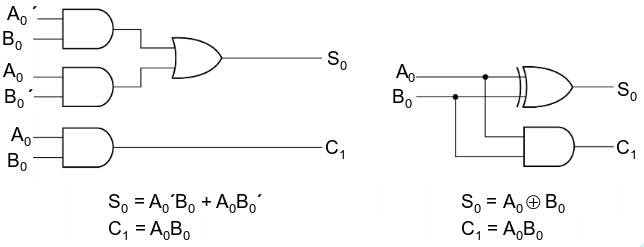
\includegraphics[scale = 0.7]{halvadd.jpg}
		\caption{Halvadder implementasjon}
	\end{figure}
	
	\subsubsection*{Fulladder:}
	Fulladder tar mente inn.
	
	Fulladder implementasjon
	\begin{figure}[H]
		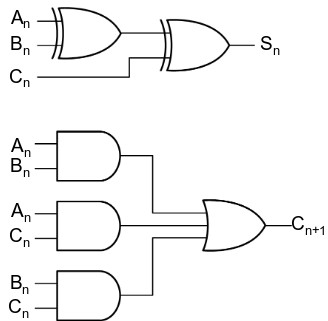
\includegraphics[scale = 0.7]{Fulladd.jpg}
		\caption{Fulladder implementasjon}
	\end{figure}
	
	\subsubsection*{Et adder system}
	\begin{figure}[H]
		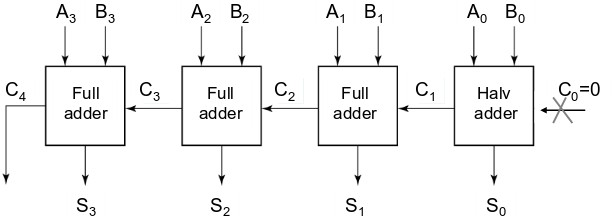
\includegraphics[scale = 0.6]{adderment.jpg}
		\caption{Et system av halv og fulladdere}
	\end{figure}
	
	\begin{figure}[H]
		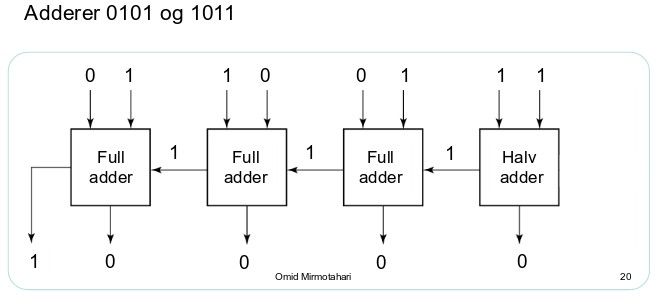
\includegraphics[scale = 0.6]{addeks.jpg}
		\caption{Et eksempel på addisjon av to binære 4-bits tall}
	\end{figure}
	
	\subsection*{”Carry Lookahead”}
	 Ønsker å unngå menteforplantning – gir økt hastighet
	 
	 $G_i$ – generate: brukes i menteforplantningen
	 $P_i$ – propagate: påvirker menteforplantningen
	
	\subsection*{Komparator:}
	Komparator – sammenligner to tall A og B 
	
	$3 utganger: A=B, A>B og A<B$
	
	\begin{figure}[H]
		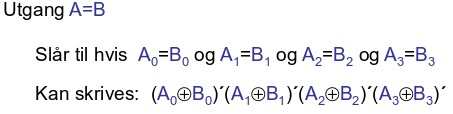
\includegraphics[scale = 0.6]{komp1.jpg}
		\caption{A=B}
	\end{figure}
	
	
	\begin{figure}[H]
		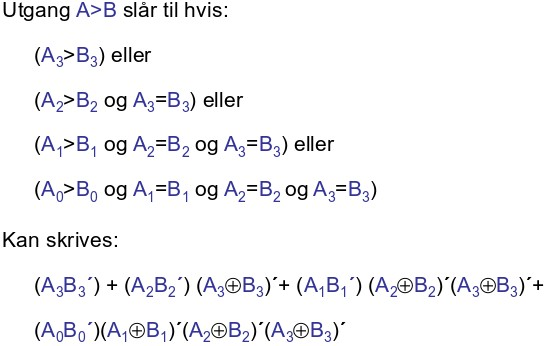
\includegraphics[scale = 0.6]{komp2.jpg}
		\caption{$A>B$}
	\end{figure}
	
	\begin{figure}[H]
		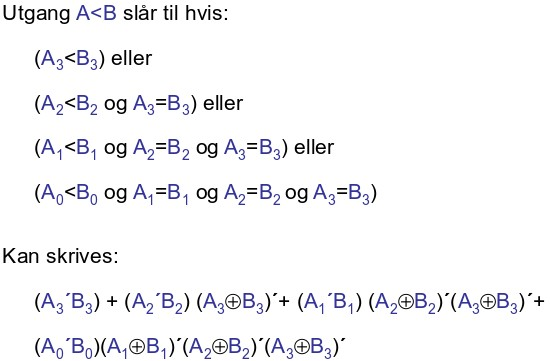
\includegraphics[scale = 0.6]{komp3.jpg}
		\caption{$A<B$}
	\end{figure}
	
	\subsection*{Dekoder:}
	 Dekoder – tar inn et binært ord og gir ut alle mintermer 
	 Kan generere generelle logiske funksjoner direkte fra mintermene på utgangen 
	 Eksempel: 3bit inn/8bit ut 
	 
	\begin{figure}[H]
		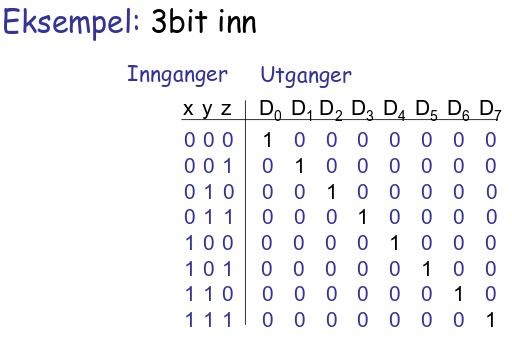
\includegraphics[scale = 0.6]{decoder.jpg}
		\caption{Sannhetstabell til en 3 bits decoder}
	\end{figure}
	
	\subsection*{Enkoder:}
	Enkoder er motsatt av dekoder
	
	\begin{figure}[H]
		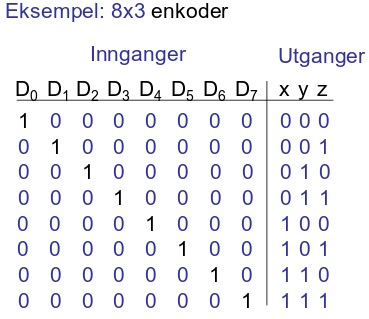
\includegraphics[scale = 0.6]{enkoder.jpg}
		\caption{Sannhetstabell for en 8x3 enkoder}
	\end{figure}
	
	Prioritets-enkoder:
	
	Hvis flere ”1”ere inn - ser kun på inngang med høyst indeks (prioritet) 
	
	
	\subsection*{Multiplekser (MUX):}
	Velger hvilke  innganger som slippes ut
	
	\begin{figure}[H]
		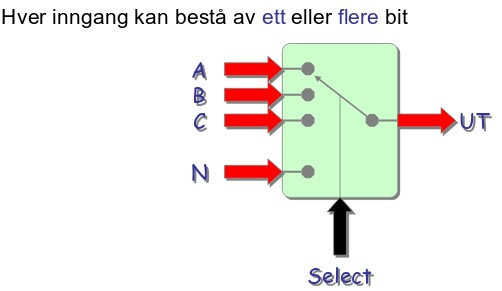
\includegraphics[scale = 0.6]{MUX.jpg}
		\caption{MUX}
	\end{figure}
	
	\begin{figure}[H]
		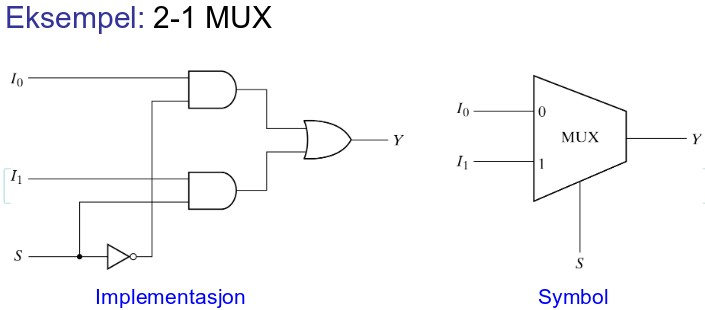
\includegraphics[scale = 0.6]{MUX2.jpg}
		\caption{En 2-1 MUX}
	\end{figure}
	
	
	\subsection*{Demulitplekser:}
	Motsatt av MUX, velger hvilke utganger som slippes ut
	
	\begin{figure}[H]
		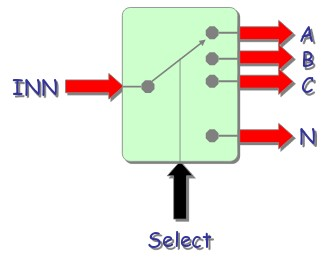
\includegraphics[scale = 0.6]{DEMUX.jpg}
		\caption{Demultiplekser}
	\end{figure}
	
	
	\subsection*{Aritmetisk logisk enhet (ALU):}
	En elektronisk krets som utfører aritmetiske og logiske operasjoner	
	
	\section*{Sekvensiell logikk:}
	
	Kombinatorisk logikk:
	Utgangsverdiene er entydig gitt av nåværende kombinasjon av inngangsverdier.
	
	Sekvensiell logikk:
	Inneholder hukommelse (låsekretser) Utgangsverdiene er gitt av nåværende kombinasjon av inngangsverdier,  samt sekvensen av tidligere inngangs-­/utgangsverdier.
	
	
	
	\section*{Tilstandsmaskiner:}
	
	\section*{Datamaskinarkitektur:}
	
	\section*{CMOS}
		
			
\end{document}